\section{Analyse des maillages}
Dans un premier temps, nous allons analyser les maillages qui nous a été fourni. L'analyse des maillages est important pour estimer la finesse des résultats obtenus et la vitesse à laquelle un résultat acceptable sera obtenu. Nous ferons donc attention aux points suivants :
\begin{itemize}
	\item Les zones où le maillage sera plus resseré (ou plus lâche)
	\item La structure du maillage
	\item La taille des mailles
\end{itemize}

\subsection{Maillage de la cabine seule}
\begin{figure}[!h]
\centering
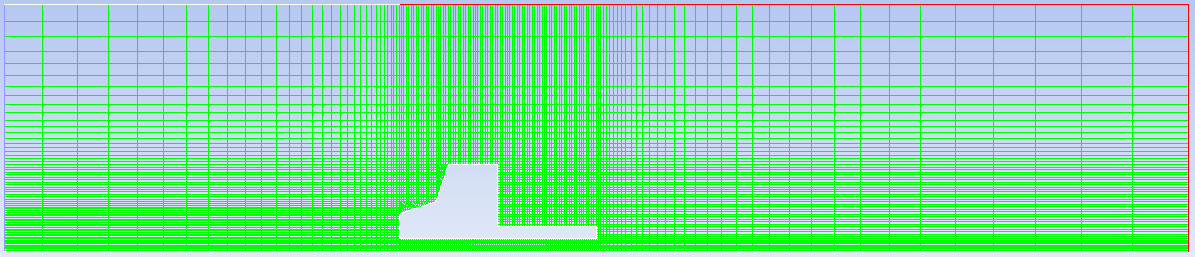
\includegraphics[scale=0.4]{images/camion_cabine_1.png}
\caption{1\ier{} maillage : camion sans remorque}
\end{figure}
On remarque que le maillage est très fin en dessous du camion, mais très large à l'avant et à l'arrière. Cela peut en effet poser quelques problèmes : on imagine facilement qu'il doit y avoir normalement plus de perturbations à l'avant et à l'arrière du camion (ou en tout cas à proximité des parois). Les résultats seront donc d'autant moins précis dans les zones qui pourraient nous intéresser.\\
Dans cet exemple, le volume des mailles vont de $10^{-3}$ à 1,5, ce qui peut sembler acceptable dans l'ensemble. On détail peut cependant paraître génant : le maillage n'est pas structuré. On remarque en effet des triangles au niveau du capot, alors que tout le reste est maillé avec des quadrilatères. Sol et plafond à gauche sont également définis de manière étrange : les frontières ont la même structure en ces endroits (deux murs par défaut). Il aurait pu être intéressant de pouvoir modifier indépendament ces deux frontières.

\subsection{Maillage avec cabine à la même hauteur que la remorque}
%Clément, boulot !
Ce maillage semble ici plutôt bien défini dans l'ensemble. Contrairement au précédent, il est relativement fin dans les endroits utiles (au contact du camion, avant, arrière et en dessous). On remarque cependant un problème présent dans tous les maillages par rapport aux roues. en effet, comment peut-on modéliser l'écoulement du vent influencé par les roues ? Ce problème n'est pas réglable sans 3D. On pourrait par exemple définir une sorte de frontière perméable qui ne laisse passer qu'une partie des flux, mais il serait assez difficile de bien mesurer l'influence à accorder à ces parois.\\
Dans ce maillage, les mailles ont un volume compris entre $3.10^{-7}$ et 1,5. Le volume minimal peut sembler un peu faible mais ne devrait pas poser de problème à Fluent. Le tout est structuré en quadrilatères.

\subsection{Maillage avec cabine de hauteur inférieure à la remorque}
\begin{figure}[!h]
\centering
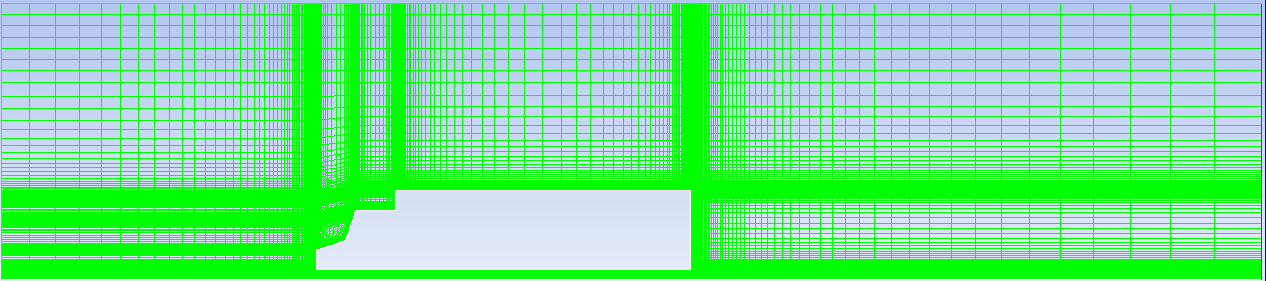
\includegraphics[scale=0.38]{images/camion_remorque_1.png}
\caption{3\ieme{} maillage : camion avec une remorque de hauteur supérieure à la cabine}
\end{figure}
On remarque ici que le maillage est organisé en plusieurs blocs, ce qui est plutôt une bonne chose car il permet des calculs rapides dans l'ensemble mais précis dans les zones où les écoulements seront plus perturbés (près du camion par exemple). Mais le résultat semble étrange : pourquoi le maillage est-il si resserré à l'avant, et pas autant à l'arrière ? Surtout qu'on peut imaginer que le flux sera d'autant plus perturbé à l'arrière sur une longue distance mais pas tellement à l'avant du camion, à part très près des parois. On aurait également pu le relâcher un peu plus en hauteur, mais cela aurait généré des mailles non perpendiculaires, ce qui peut compliquer les calculs (mais ce qui ne semble pas être un problème pour Fluent). Cependant, le fait que le maillage soit très fin au niveau des parois reste tout de même une bonne chose, surtout au dessus de la cabine où les petits coins formés avec la remroque seront très probablement source de tourbillons. \\
Les mailles ont ici un volume entre $10^{-7}$ et 1,6, ce qui ne semble pas être gênant lors de nos calculs.

\subsection{Maillage avec cabine de hauteur supérieure à la remorque}
%Clément, boulot !

\section{Analyse des résultats obtenus}
Maintenant que nos maillages ont été commentés et analysés, nous allons regarder les résultats obtenus lors de nos phases de calcul. Cependant, avant de lancer les calculs, quelques paramètres ont dû être reglés afin d'assurer une certaine convergence des calculs et surtout pour obtenir des résultats assez réalistes :
\begin{itemize}
	\item On remarque que le nombre de Reynolds est ici à $3.10^6$ à $60$ hm.h$^{-1}$. Étant donné que ce nombre est supérieur à $500$ $000$, on va consédérer cet écoulement commme non laminaire. \\%On reparle de comment on calcul ce nombre ou pas ?
On retrouve le même résultat à 110 km.h$^{-1}$. 
	\item Le modèle choisi ici est le modèle k-epsilon de Fluent. %Oui, mais, pourquoi celui-là en fait ?
Étant donné qu'on a un obstacle (ce qui est tout de même le c\oe ur de notre analyse), on choisit le modèle RNG pour obtenir plus de précision.
	\item Au niveau des différentes entrées, on doit également régler bien évidemment la vitesse (sans oublier de la mettre en m.s$^{-1}$) ainsi que la turbulance (étant donné qu'on a demandé un modèle turbulant). On a ici deux paramètres à régler ($K$ et $\varepsilon$), mais nous allons plutôt donner deux autres paramètres pour permettre à Fluent de calculer automatiquement ces paramètres de modèle :
	\begin{itemize}
		\item[$\bullet$] On règle tout d'abord la \textit{turbulent intensity} (en \%), qui est automatiquement reglé sur 10\% et qui semblerait être le meilleur taux qu'on puisse utiliser
		\item[$\bullet$] On règle ensuite le \textit{turbulent length scale} (en m) qui correspond à une échelle à laquelle on estime l'influence de la perturbation autour de notre obstacle. %Really ?
On le règle ici à 3m.
	\end{itemize}
\end{itemize}

\bigskip
On étudiera ici plusieurs résultats :
\begin{itemize}
	\item les lignes de courant et les champs de pression et de vitesse
	\item les coefficients de frottement avec les parois
\end{itemize}

\subsection{Étude de la cabine seule}
\begin{figure}[!h]
\centering
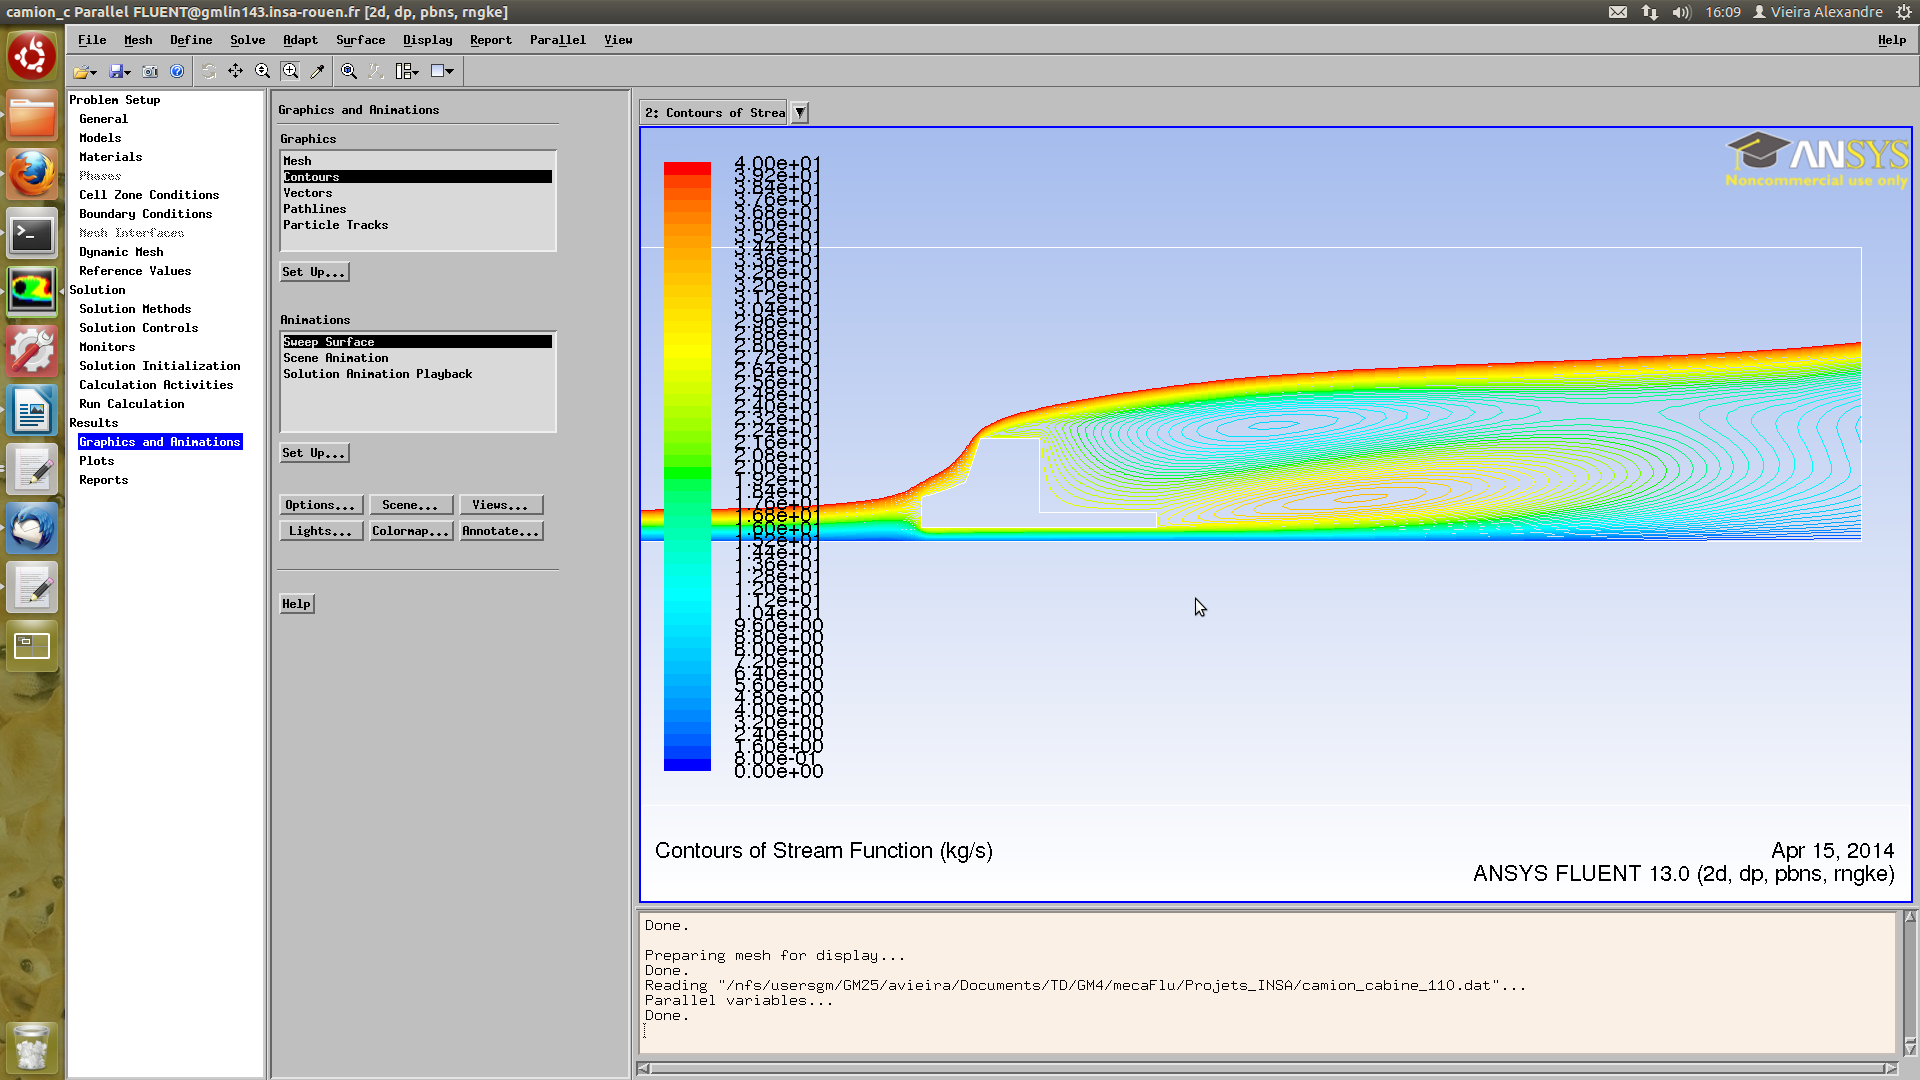
\includegraphics[scale=0.4]{resultsCx/camion110_stream.png}
\caption{Lignes de courant pour la cabine seule à 110 km.h$^{-1}$}
\label{figCabStream110}
\end{figure}
On commence par étudier les lignes de courant présentés figure \ref{figCabStream110}. Les résultats ne sont présentés ici qu'à 110 km.h$^{-1}$ car ils changent très peu à 60 km.h$^{-1}$. \\
On remarque ici très clairement la traînée laissée par le camion lors de son passage. A l'arrivée sur le camion, le vent suit très clairement deux chemins : soit par le capot et au dessus du camion, soit par en dessous. Il en resulte juste derrière la cabine un tourbillon qui semble persister. On le voit plus clairement avec les vecteurs vitesse présentés figure \ref{figCabVit110}.

\begin{figure}[!h]
\centering
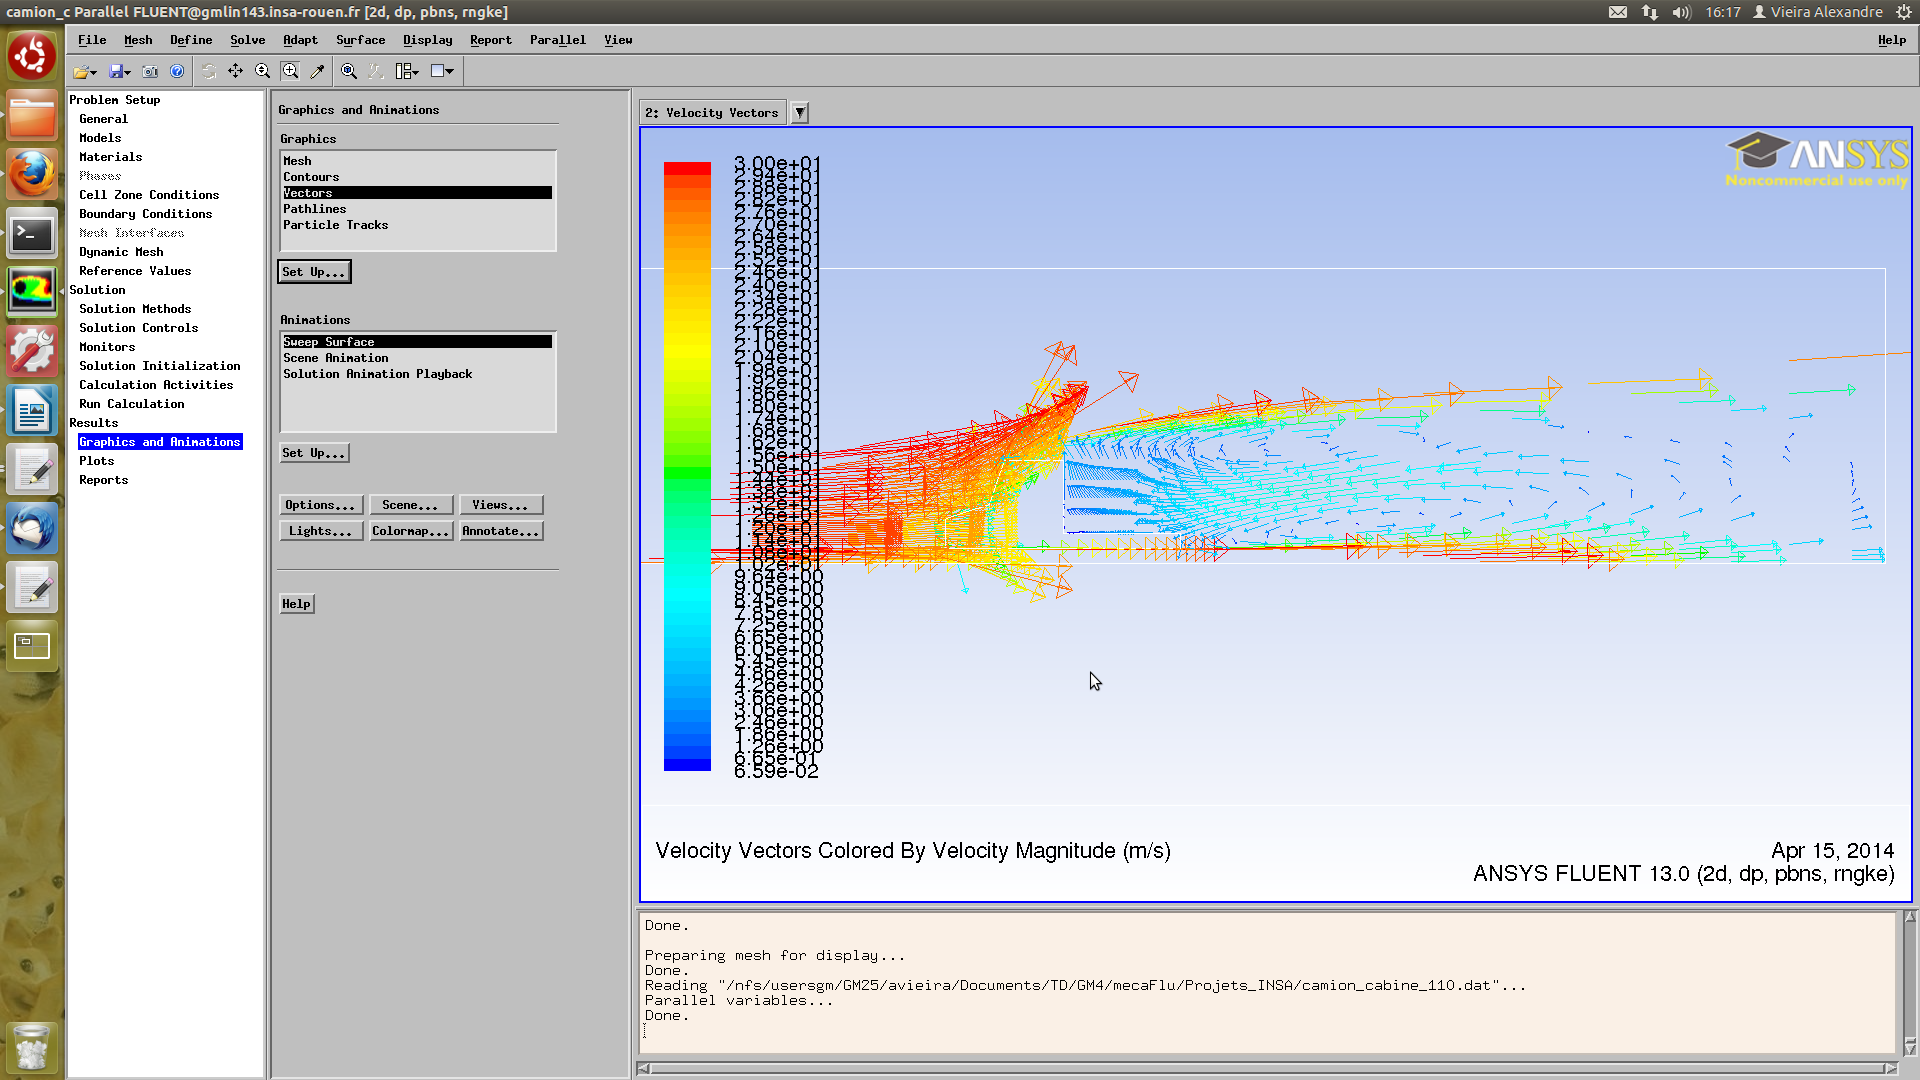
\includegraphics[scale=0.4]{resultsCx/camion110_velocityVectors.png}
\caption{Vecteurs vitesse pour la cabine seule à 110 km.h$^{-1}$}
\label{figCabVit110}
\end{figure}
\clearpage

Étudions à présent la pression sur les parois du camion. Comme on peut le voir figure \ref{figCabPres110}, on a une pression plus faible à l'arrière de la cabine comparé à l'avant. Cela entraîne une sorte de resistance à l'avancement du camion.
\begin{figure}[!h]
\centering
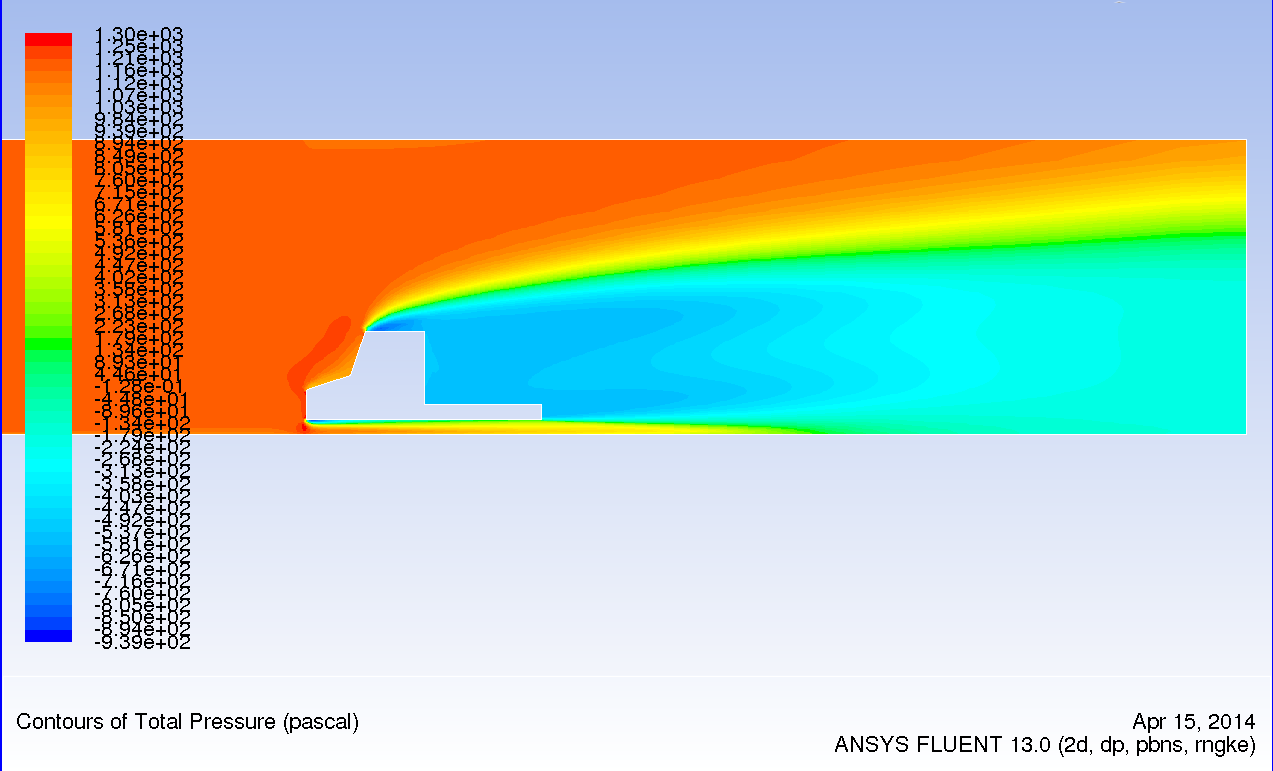
\includegraphics[scale=0.4]{resultsCx/camion110_pressure.png}
\caption{Champ de pression pour la cabine seule à 110 km.h$^{-1}$}
\label{figCabPres110}
\end{figure}

On peut également observer les coefficients de frottement contre les parois suivant les vecteurs de la base canonique (bien nommés coefficients Cx et Cy). Les parois qui nous intéresseront seront bien sûr les parois du camion et non pas tous les autres murs qui définissent la frontière du domaine. \\
On a ici deux données pour les frottements qui sont exprimés en Newton : une mesure Pressure qui donne la force de pression normale à la surface, et une mesure Viscous qui nous donne les frottements tangentiels. Il peut être intéressant de regarder la proportions de forces tangentiels par rapport aux forces totales : si la proportion est forte, il pourrait être intéressant de reserrer le maillage près des parois pour connaître plus précisément la forme des écoulements.\\
Les résultats sont dans cet exemple les suivants :
\begin{center}\begin{tabular}{|l|r r r|}
\hline
\multicolumn{4}{|c|}{Forces - Direction Vector (1 0 0)} \\
\hline
		&   \multicolumn{3}{c|}{Forces (n)} \\
\hline
Zone                &     Pressure    &   Viscous     &   Total      \\
\hline
arriere\_cabine      &     1353.4712   &   0           &   1353.4712  \\
arriere\_camion     &      272.26549   &   0           &   272.26549  \\ 
capot               &     415.56441    &  1.5682516    &  417.13266   \\
pare-brise          &     1048.325     &  0.98624219   &  1049.3113   \\
pare-bufle          &     1121.3655    &  0            &  1121.3655   \\
plancher            &     0            &  20.532769    &  20.532769   \\
plateau             &     0            &  -0.50339391  &  -0.50339391 \\
toit                &     0            &  -1.7254131   &  -1.7254131  \\
\hline
\hline
Net                 &     4210.9917    &  20.858455    &  4231.8501   \\
\hline
\end{tabular}\end{center}

\begin{center}\begin{tabular}{|l|r r r|}
\hline
\multicolumn{4}{|c|}{Forces - Direction Vector (0 1 0)} \\
\hline
		&   \multicolumn{3}{c|}{Forces (n)} \\
\hline
Zone                &     Pressure    &   Viscous     &   Total      \\
\hline
arriere\_cabine      &     0           &   0.24353637  &   0.24353637  \\ 
arriere\_camion      &     0           &   -0.090688751&   -0.090688751\\ 
capot               &     -1246.6932  &   0.52275052  &   -1246.1705  \\ 
pare-brise          &     -349.44168  &   2.9587266   &   -346.48295  \\ 
pare-bufle          &     0           &   -0.48552695 &   -0.48552695 \\ 
plancher            &     -4611.9409  &   0           &   -4611.9409  \\ 
plateau             &     2179.7929   &   0           &   2179.7929   \\ 
toit                &     1747.0896   &   0           &   1747.0896   \\ 
\hline
\hline
Net                 &     -2281.1934  &   3.1487978   &   -2278.0446  \\ 
\hline
\end{tabular}\end{center}

On voit ici que les forces tangentielles sont clairement faibles par rapport aux forces totales. Il n'est donc nul besoin de resserer le maillage.\\
Par rapport aux forces en elles-mêmes, on retrouve l'aspiration à l'arrière du camion qui empêche le camion d'avancer, au même niveau que le tourbillon. Le vent oppose également une certaine resistance à l'avancement du camion en exerçant une pression sur le capot, le pare-brise et le pare-bufle. 
%Parler dessous camion.

\subsection{Étude avec cabine à la même hauteur que la remorque}

\subsection{Étude avec cabine de hauteur inférieure à la remorque}
Les lignes de courant montrés dans la figure \ref{figRem2Stream110} montrent encore un tourbillon à l'arrière du camion ainsi que vers le capot. Cependant, on remarque en plus un petit tourbillon supplémentaire au dessus de la cabine, devant la remorque. \\ 

\begin{figure}[!h]
\centering
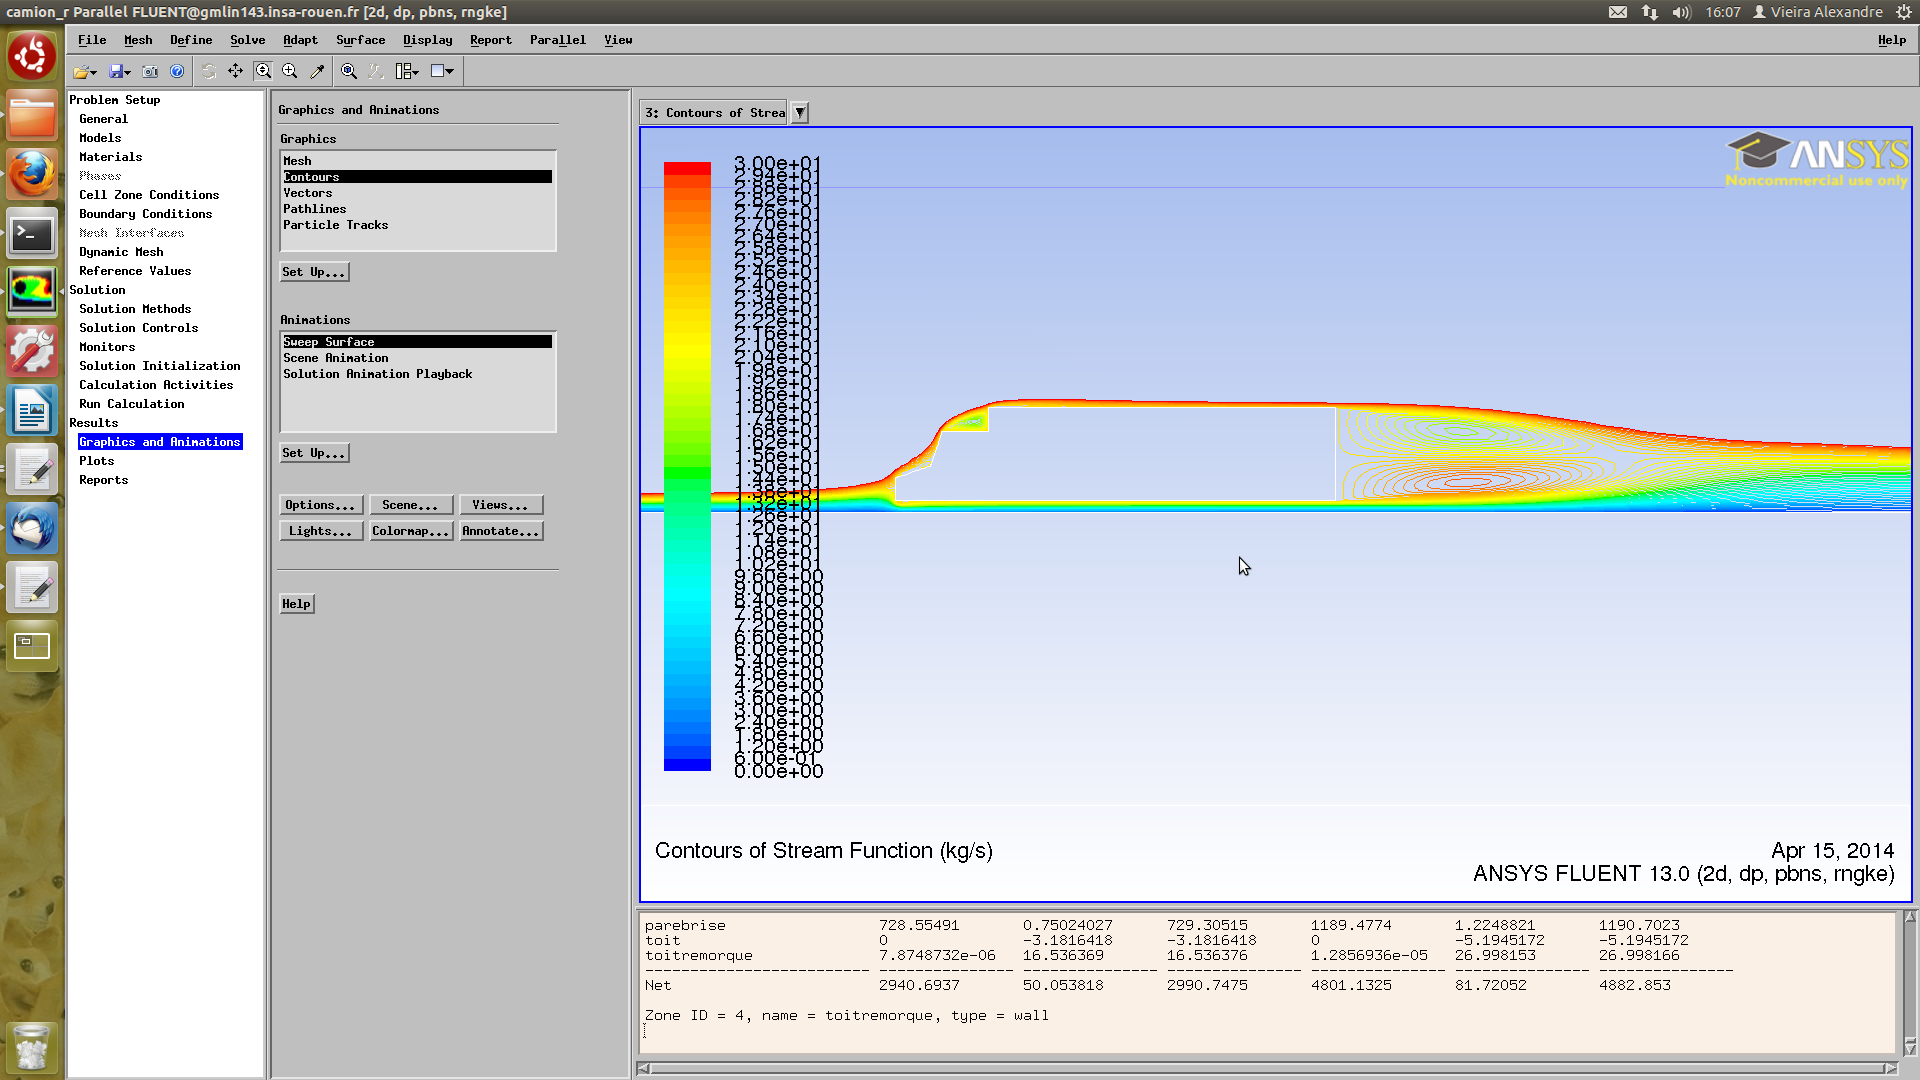
\includegraphics[scale=0.4]{resultsCx/remorque2_110_stream.png}
\caption{Lignes de courant pour le camion avec remorque plus grande à 110 km.h$^{-1}$}
\label{figRem2Stream110}
\end{figure}
\clearpage

On étudie ces tourbillons de plus près grâce aux vecteurs vitesse figure \ref{figRem2Vit110} et surtout grâce à la figure \ref{figRem2Vit110-coin}. La première nous montre le même tourbillon que vu précédemment. La deuxième figure nous montre un petit tourbillon qui se forme juste au-dessus de la cabine dû au fait que la remorque est plus haute que la cabine.\\
\begin{figure}[!h]
\centering
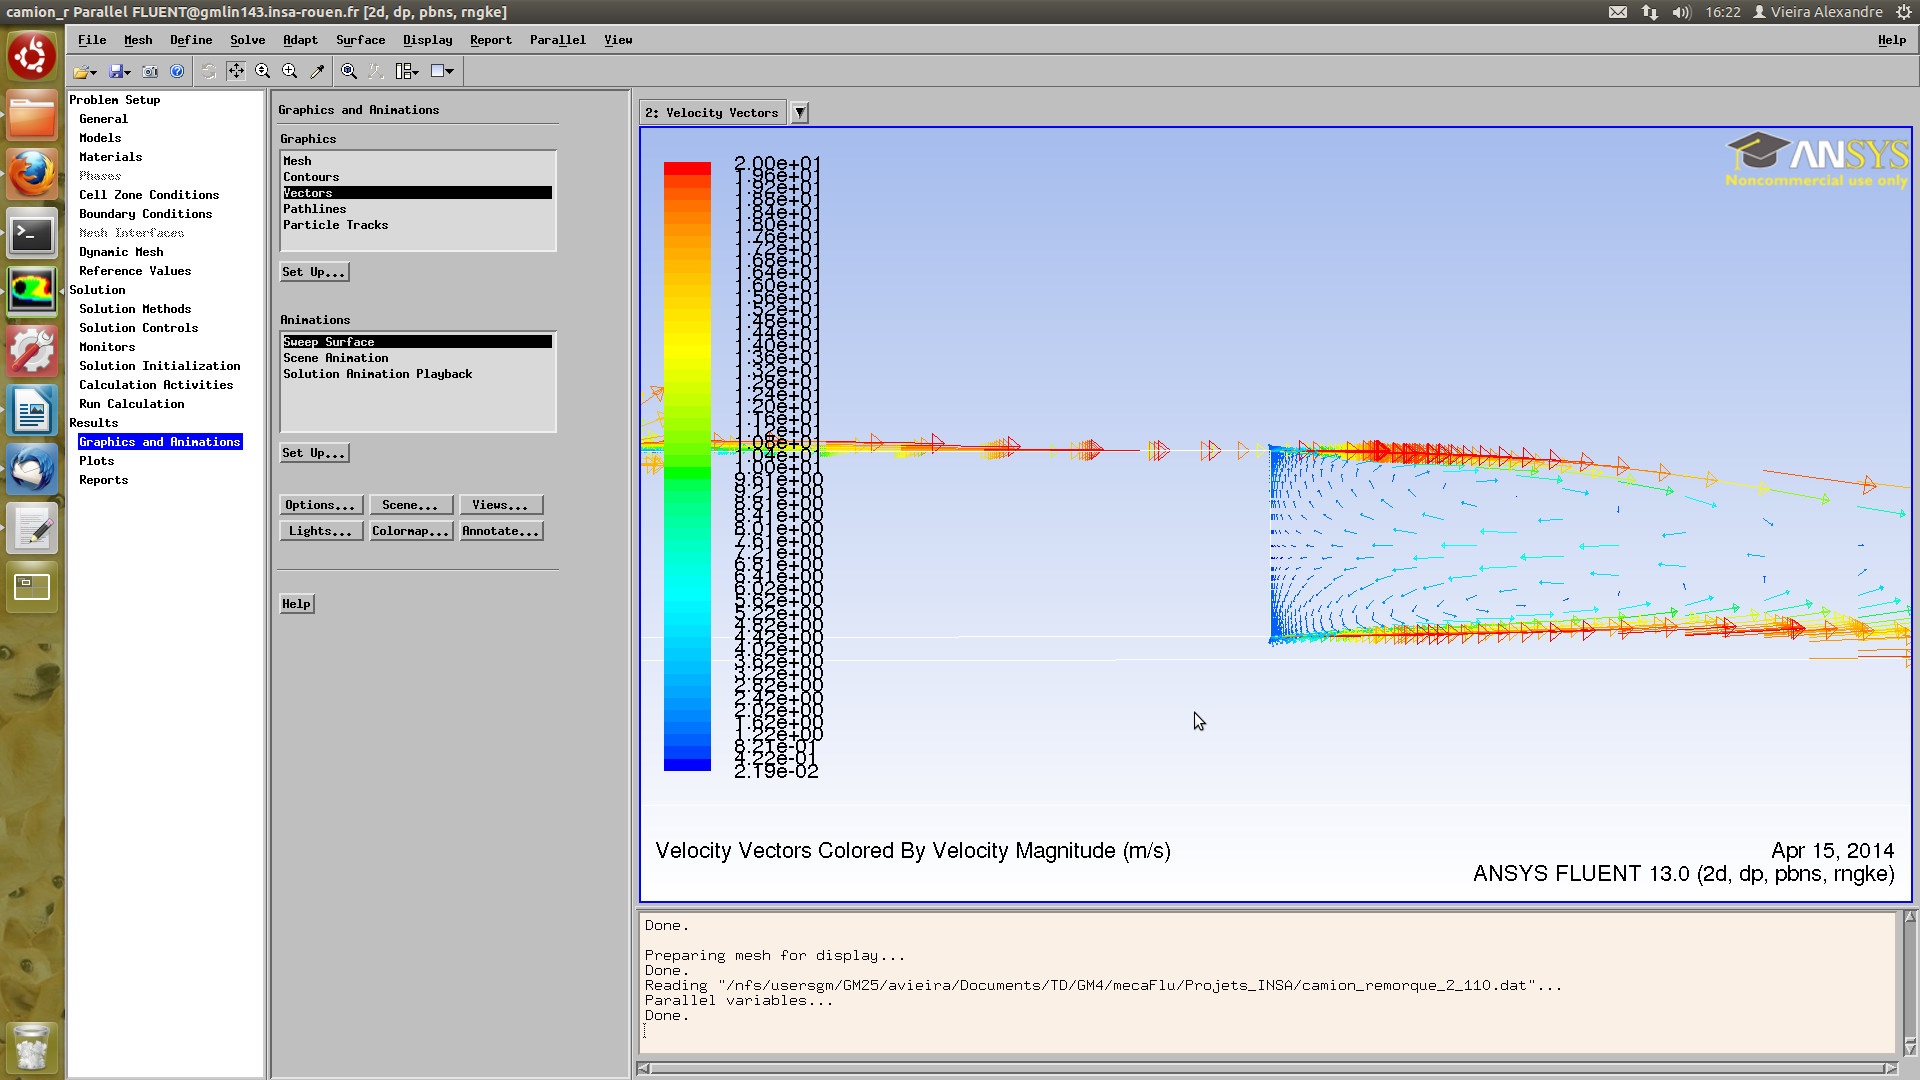
\includegraphics[scale=0.4]{resultsCx/Remorque2-110_VelocityVectors.png}
\caption{Vecteur vitesse pour le camion avec remorque plus grande à 110 km.h$^{-1}$}
\label{figRem2Vit110}
\end{figure}
\begin{figure}[!h]
\centering
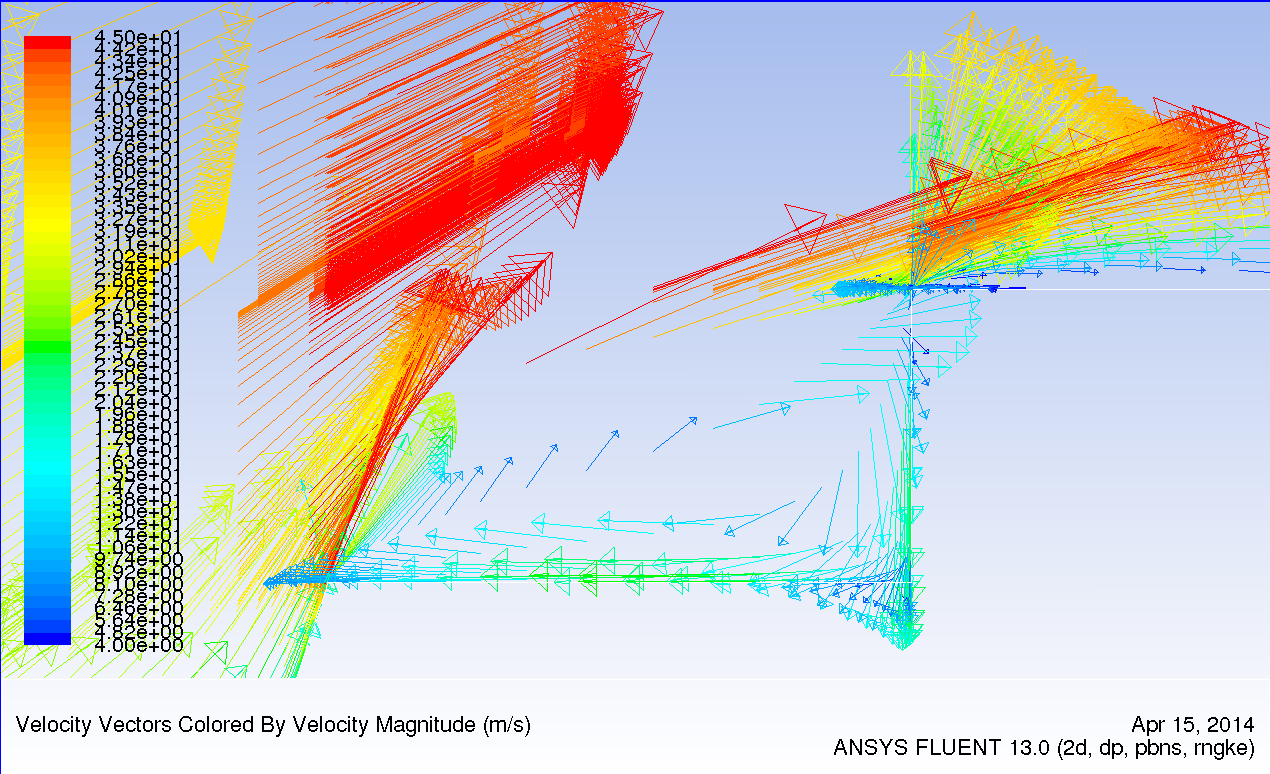
\includegraphics[scale=0.4]{resultsCx/remorque2-hautCabineAbsorption.png}
\caption{Vecteur vitesse dans le coin entre le haut de la cabine et l'avant de la remorque.}
\label{figRem2Vit110-coin}
\end{figure}
\clearpage

Ce dernier pourrait sembler banal, mais on remarque en étudiant les pressions qu'il pourrait en vérité aider (un minimum) le camion à avancer. En effet, si on regarde le champ de pression figure \ref{figRem2Pres110} et surtout les coefficients de frottement, on se rend compte de ce résultat.
\begin{figure}[!h]
\centering
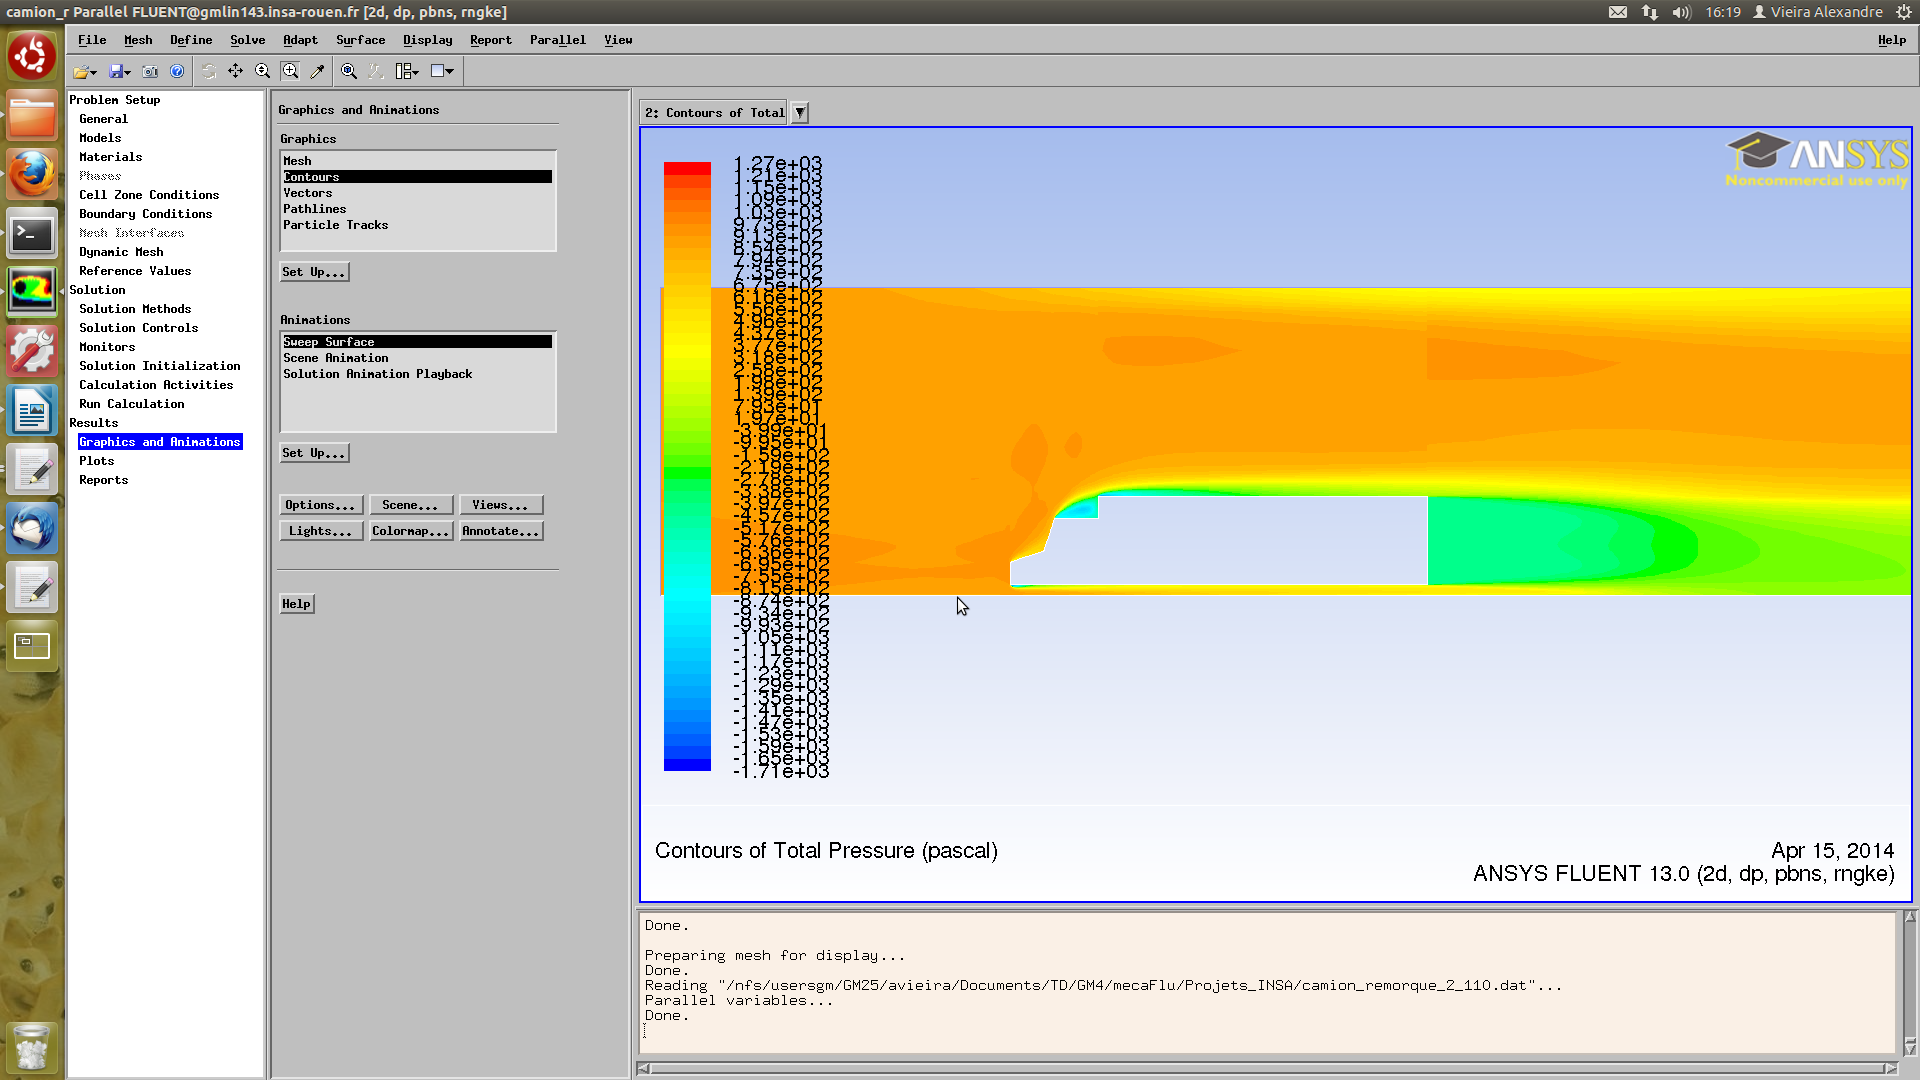
\includegraphics[scale=0.4]{resultsCx/remorque2-110_pressure.png}
\caption{Champ de pression pour le camion avec remorque plus grande à 110 km.h$^{-1}$}
\label{figRem2Pres110}
\end{figure}

\begin{center}\begin{tabular}{|l|r r r|}
\hline
\multicolumn{4}{|c|}{Forces - Direction Vector (1 0 0)} \\
\hline
                     &    \multicolumn{3}{c|}{Forces (n)} \\                                
\hline
Zone                 &    Pressure       & Viscous        & Total     \\ 
\hline
arriere              &    1737.1378      & 0              & 1737.1378 \\ 
avant                &    854.85113      & 0              & 854.85113 \\ 
avantremorque        &    -643.02092     & 3.0323539e-08  & -643.02092\\ 
bas                  &    0              & 36.397427      & 36.397427 \\ 
capot                &    263.17073      & -0.44857616    & 262.72215 \\ 
parebrise            &    728.55491      & 0.75024027     & 729.30515 \\ 
toit                 &    0              & -3.1816418     & -3.1816418\\ 
toitremorque         &    7.8748732e-06  & 16.536369      & 16.536376 \\ 
\hline
\hline
Net                  &    2940.6937      & 50.053818      & 2990.7475 \\ 
\hline
\end{tabular}


\begin{tabular}{|l|r r r|}
\hline
\multicolumn{4}{|c|}{Forces - Direction Vector (0 1 0)} \\
\hline
                        &  \multicolumn{3}{c|}{Forces (n)} \\
\hline
Zone                    & Pressure      &  Viscous       &  Total      \\ 
\hline
arriere                 & 0             &  0.015144547   &  0.015144547\\
avant                   & 0             &  -0.42331351   &  -0.42331351\\
avantremorque           & -1.2852065e-05&  -1.5135782    &  -1.513591  \\
bas                     & -7194.5353    &  0             &  -7194.5353 \\
capot                   & -789.51218    &  -0.14952539   &  -789.6617  \\
parebrise               & -242.85164    &  2.2507208     &  -240.60092 \\
toit                    & 1850.4328     &  0             &  1850.4328  \\
toitremorque            & 7879.9682     &  -1.653932e-08 &  7879.9682  \\
\hline
\hline
Net                     & 1503.5019     &  0.17944826    &  1503.6813  \\
\hline
\end{tabular} \end{center}

On voit donc que les efforts sur l'avant de la remorque sont opposés à ceux à l'arrière. Une légère dépression qui permet au camion d'avancer un peu plus facilement ! 

\subsection{Étude avec cabine de hauteur supérieure à la remorque}

\section{Commentaires}
